\documentclass[a4paper,oneside,12pt]{article}

\usepackage[utf8]{inputenc}
\usepackage[T1]{fontenc}
\usepackage[french]{babel}
\usepackage{hyperref}
\usepackage{listings}
\usepackage{listingsutf8}

\newcommand{\airplug}{AIRPLUG}
\newcommand{\pie}{PIE}
\newcommand{\timestamp}{\textit{timestamp}}
\newcommand{\mdcinq}{MD5}
\newcommand{\hash}{\textit{hash}}

\newcommand{\chrisb}{Christophe Boudet}
\newcommand{\julien}{Julien Castaigne}
\newcommand{\chrisr}{Christophe Roquette}
\newcommand{\joe}{Jonathan Roudière}
\newcommand{\jeremy}{Jérémy Subtil}

\newcommand{\format}[1]{\begin{description}\item[Format] \texttt{#1}\end{description}}
\newcommand{\formatvar}[2]{\begin{description}\item[Format] \texttt{#1}~$\Rightarrow$ \texttt{#2}\end{description}}
\newcommand{\apgcmd}[1]{\texttt{#1}}
\newcommand{\fcmd}[2]{\texttt{#1\apgeq#2}}
\newcommand{\fkcmd}[1]{\texttt{#1}}
\newcommand{\fvcmd}[1]{\texttt{<#1>}}
\newcommand{\msgcmd}[1]{\texttt{#1}}



\newcommand{\customtitle}{Projet SR05 -- Réalisation d'une application répartie sur la plateforme \airplug}
\newcommand{\customsubject}{\pie}

\title{\customtitle}
\author{\chrisb, \julien, \chrisr,\\\joe, \jeremy}

\hypersetup{
	pdftitle={\customtitle},
	pdfauthor={\chrisb, \julien, \chrisr, \joe, \jeremy},
	pdfsubject={\customsubject}
}

\lstdefinelanguage{algorithme}
{keywords={si,alors,finsi,sinon,pour,faire,finfaire,et,ou,non,envoyer,recevoir},
otherkeywords={<-},
comment=[l]//,
morecomment=[l][\bfseries]**}
\lstset{language=algorithme,
frame=single,
numbers=left,
tabsize=2,
stepnumber=2,
extendedchars=true,
numberstyle=\tiny,
basicstyle=\small,
extendedchars=true,
inputencoding=utf8/latin1}


\begin{document}

\maketitle

%mainfile: rapport.tex

\section{Algorithme réparti}

\lstinputlisting[caption={Algorithme réparti}]{algo.txt}

\subsection{Explication de l'algorithme}
\subsubsection{Initialisation}
Lors du démarrage de l'application, la base de donnée est reconstruite. Celle-ci comporte trois bases, plus une vue :
\begin{description}
	\item[bd\_abos] contient l'ensemble des identifiants de voitures, et pseudos d'utilisateurs auxquels nous sommes abonnés.
	\item[bd\_offres\_abo] contient l'ensemble des identifiants de voitures, ainsi que la distance des abonnements offerts à notre portée. Cette liste comporte des priorités, nous permettant de détruire les abonnements passagers dus à un simple croisement avec un véhicule.
	\item[bd\_demandes\_abo] a un fonctionnement identique à la base d'offres. Cependant, celui-ci intègre une partie des abonnements désirés par ces voisins.
	\item[bd\_flux] correspond à une vue des messages envoyés par nos abonnements.
\end{description}
\paragraph*{}
Un timer est ensuite enclenché afin d'effectuer à intervalle régulier un \texttt{HeartBeat}.

\subsubsection{HeartBeat}
Ce message correspond à un battement de c\oe ur, c'est à dire, une preuve d'existence. Il est diffusé à tous, mais ne pourra être relayé. Son contenu (offres et demandes du n\oe ud et de ses voisins environnants) servira à mettre à jour les bases de données des n\oe uds receveurs. Ce contenu pourra alors très bien figurer dans les messages \texttt{HeartBeat} des n\oe uds receveurs. Ce système permet de répartir la base de donnée générale des \textit{abonnements - abonnés} et ceci même lorsqu'aucun message \texttt{PIE} n'est transmis.

\paragraph*{}
Afin de former ce message, il faut tout d'abord nettoyer les bases de données. La priorité de chaque offre et demande va être décrémentée, afin que les n\oe uds que nous ne rencontrons plus aient une priorité négative. Cette priorité pourra être calculée, uniquement sur le nombre de messages \texttt{HeartBeat} de la cible, ou en prenant en compte les coordonnées GPS de celle-ci. Au contraire, à la réception d'un message, les abonnements contenus dans les offres et les demandes verront leur priorité incrémentée.

\subsubsection{Envoi et réception d'un message PIE}
Un message PIE correspond au message que l'utilisateur veut envoyer à ses suiveurs, de la même façon que sur \texttt{Tweeter}. Ce message doit donc être acheminé jusqu'à chaque voiture concernée par notre abonnement. Insérer une limite de distance dans la diffusion du message impliquerait un rayon de diffusion fixe, et ainsi, un long convoi de véhicules ne sera pas pris en compte. Augmenter la distance maximale de diffusion suppose une diffusion lointaine, probablement vers des zones n'ayant aucun intérêt pour notre abonnement. C'est pour cela que nous avons introduit deux notions : le TTL et le TTS.

\paragraph*{}
Le TTL (Time To Live) va être décrémenté chaque fois qu'une voiture retransmet le message alors que l'abonnement ne figure pas dans sa base de donnée \texttt{bd\_demandes\_abo}.
\paragraph*{}
Le TTS (Time To Survive) va être décrémenté par chaque voiture retransmettant le message alors que l'abonnement figure dans la base de donnée \texttt{bd\_demandes\_abo}.
\paragraph*{}
Un seul de ces deux compteurs peut être décrémenté. Le message n'est pas retransmis si le compteur devant être décrémenté est à 0. Ce mode de retransmission permet une diffusion intelligente. En effet, bien que le message puisse être diffusé inutilement dans un rayon égal au TTL, il pourra cependant s'étendre d'avantage dans les zones où un destinataire est présent, grâce au TTS. Le schéma ci-dessous montre ce principe.

\begin{center}
	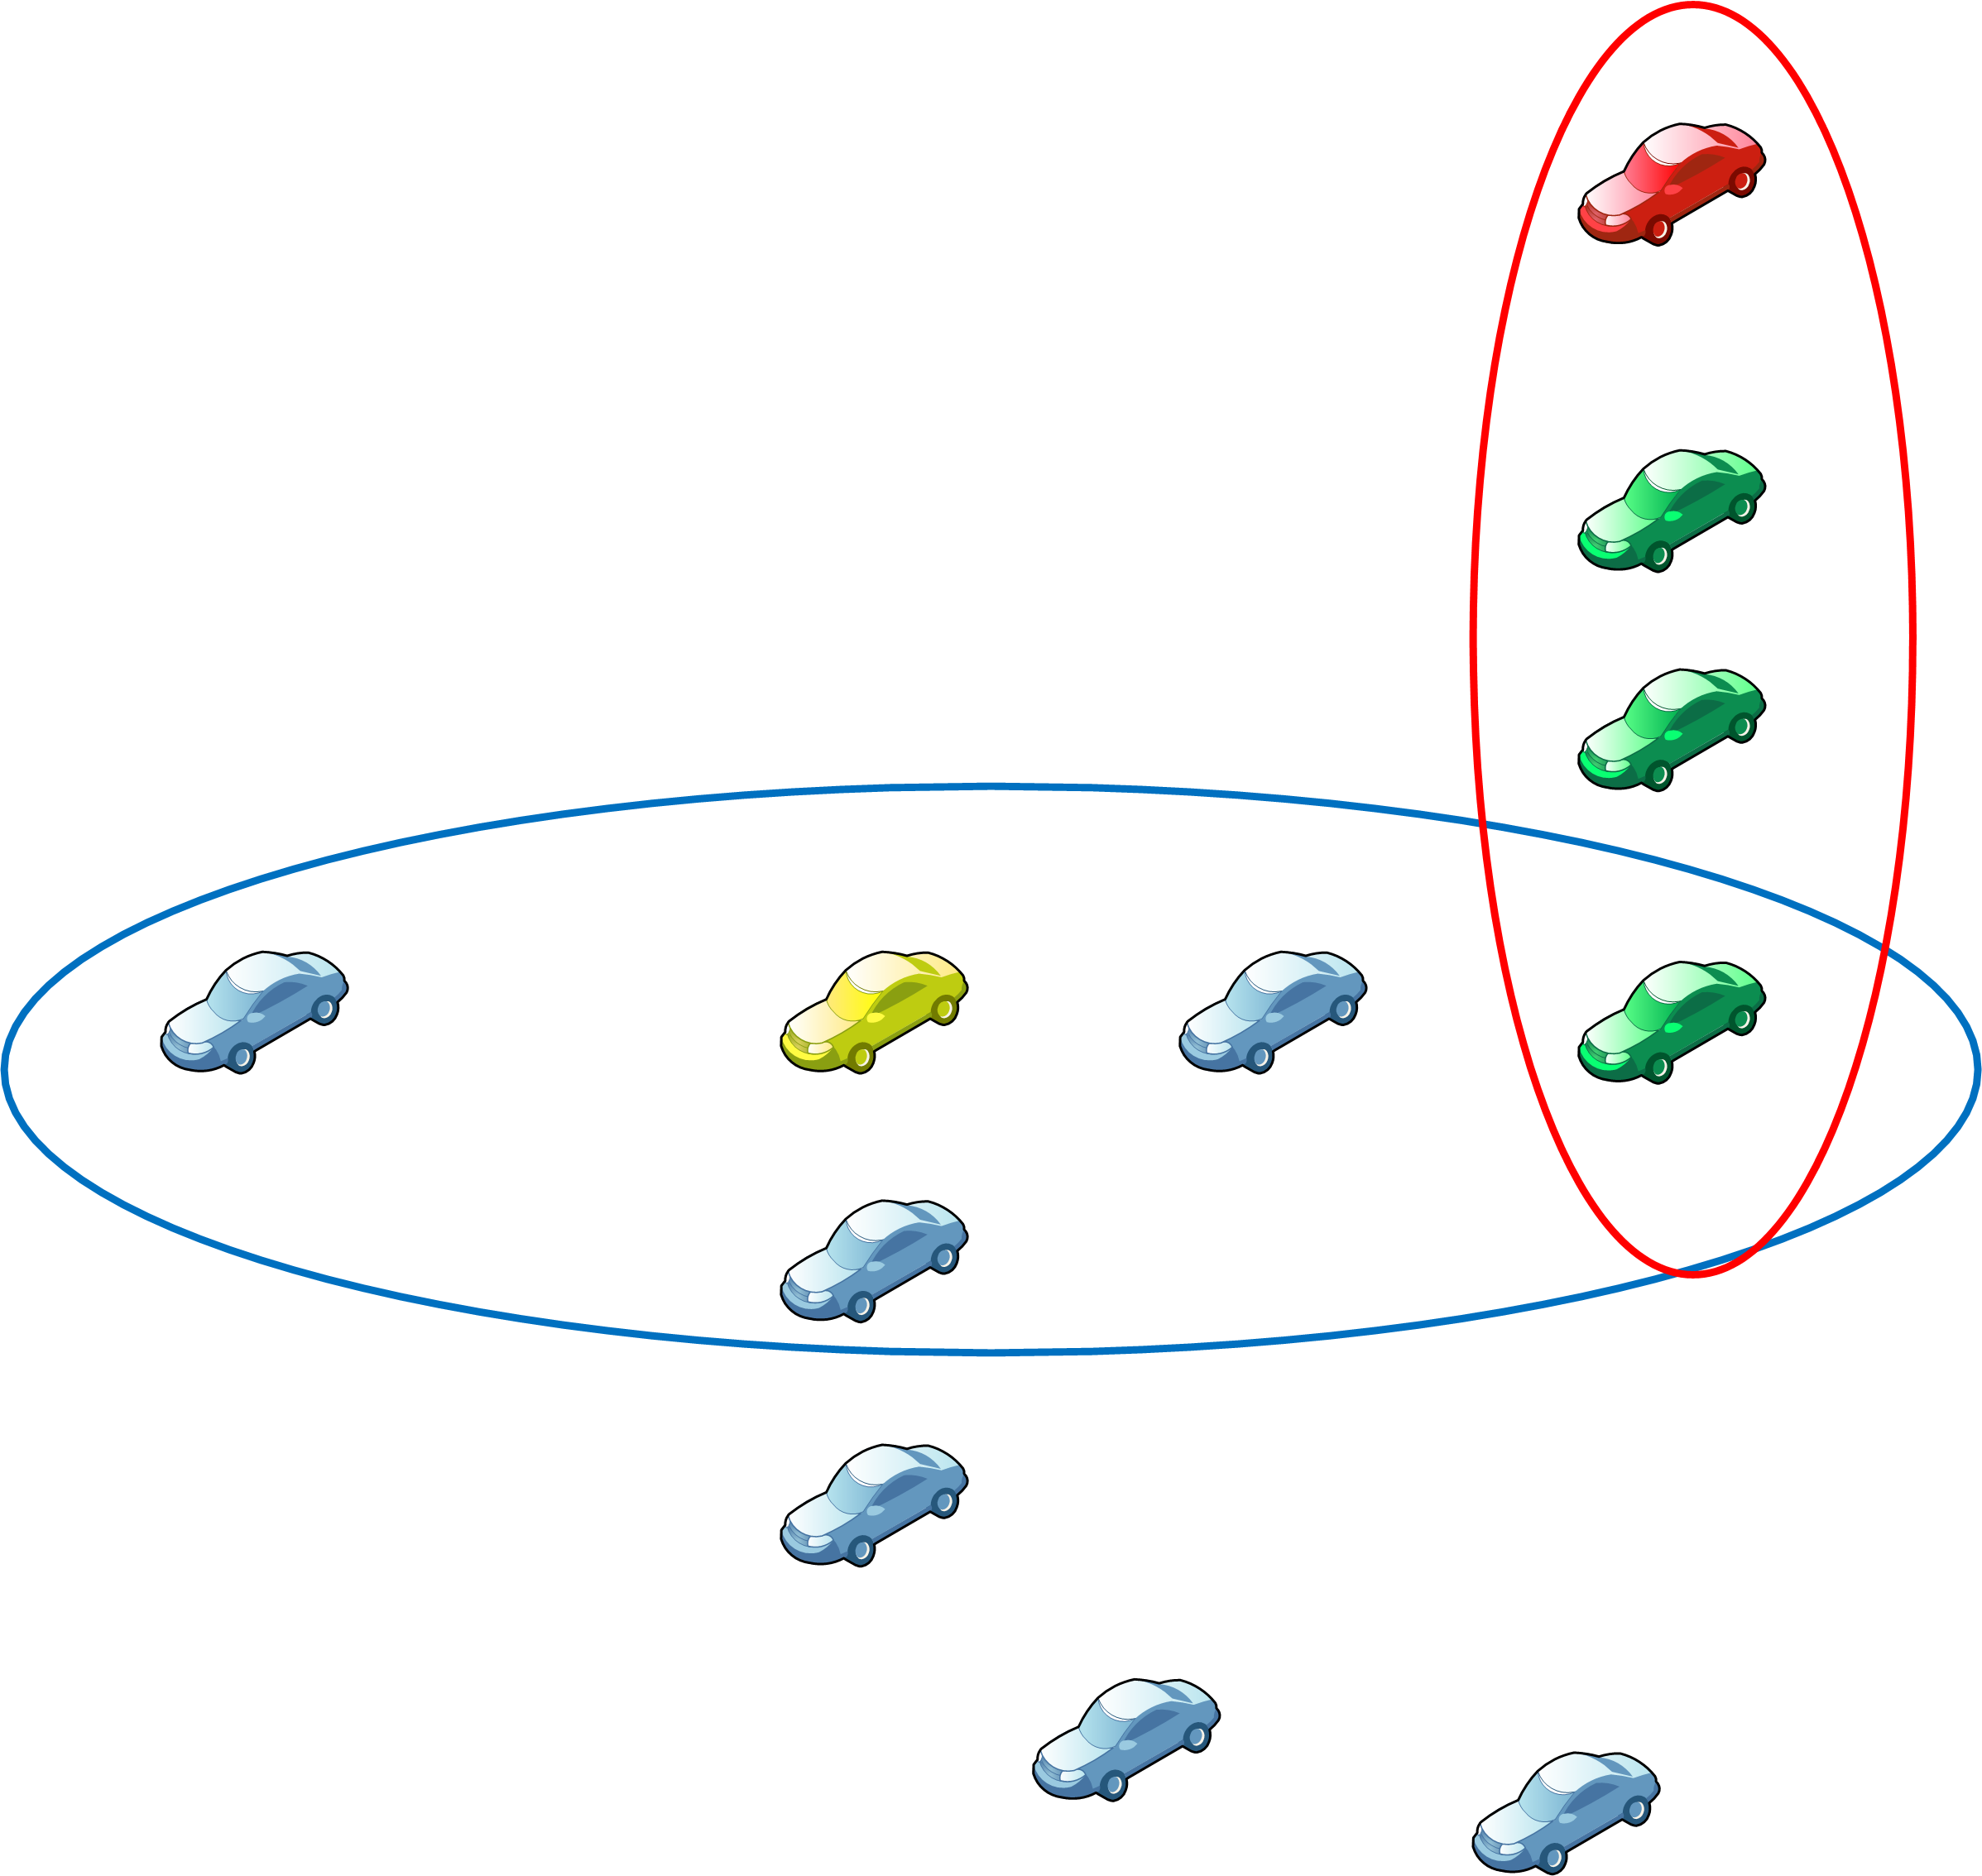
\includegraphics[width=0.75\textwidth]{img/schema2}
\end{center}

\paragraph*{}
\begin{description}
	\item[Voiture jaune :] N\oe ud émetteur du message PIE.
	\item[Voiture bleue :] N\oe ud non abonné et non intéressé par le message.
	\item[Voiture verte :] N\oe ud non abonné, mais connaissant un n\oe ud intéressé par celui-ci.
	\item[Voiture rouge :] N\oe ud abonné à l'émetteur désirant donc recevoir le message.
	\item[Ellipse bleu :] Zone de diffusion du message par décrémentation du TTL.
	\item[Ellipse rouge :] Zone de diffusion du message par décrémentation du TTS.
\end{description}
\paragraph*{}
Nous remarquons que contrairement à une diffusion par distance qui aurait un format de cercle, l'utilisation du TTL et TTS permet une diffusion ayant une forme variable. Dans le cas d'un convoi de véhicules, avec un véhicule égaré, cela va par exemple permettre de continuer à faire communiquer les deux protagonistes le plus longtemps possible.


\paragraph*{}
Dans un soucis d'optimiser chaque message, et d'avoir une convergence rapide entre les bases de données et la topologie physique de notre réseau de voitures, nous avons choisi d'inclure les offres et les demandes aux messages \texttt{PIE}. Ainsi ces messages participeront à un meilleur acheminement des futurs messages du réseau. Le réseau étant dynamique, les routes seront constamment réévaluées.


\section{Terminologie}

abonnement
message \pie
voisins


\section{Algorithme réparti et protocole}

\subsection{Identifiants}

\subsubsection{N\oe uds}

L'identifiant d'un n\oe ud est défini à l'origine par le fournisseur du produit \airplug~: c'est lui qui s'assure de leur unicité. La taille d'un tel identifiant est de 32 caractères. 


\subsubsection{Messages}

L'identifiant d'un message est définit en combinant l'identifiant du n\oe ud auteur et le \timestamp\ correspondant  à la date de sa rédaction, sur laquelle on applique l'algorithme \mdcinq. Ainsi, il s'agit d'un \hash\ de 32 caractères.


\subsection{Annonce de l'état d'un n\oe ud}

Chaque n\oe ud annonce à ses voisins, à un intervalle de temps régulier, les messages \pie\ qu'il a à offrir, ainsi que les abonnements qu'il demande.

Les offres et les demandes sont annoncées indépendamment. En effet, cette solution donne l'avantage de choisir plus finement les intervalles de temps pour chaque type d'annonce.


\subsubsection{Définition des annonces d'offre de messages}

Un n\oe ud annonce en priorité ses propres messages qu'il a à offrir. Dans une certaine limite, il annonce également les messages que ses voisins offrent de leur c\^oté.

Les messages offerts par les voisins sont pondérés avec la distance au n\oe ud courant, en nombre de sauts. En effet, les messages offerts par le n\oe ud courant sont pondérés à 0, tandis que les messages offerts par les voisins voient leur pondération d'origine incrémentée de 1.

Par exemple, les messages d'un voisin direct \texttt{A} ont une pondération de 1, alors que les messages de \texttt{B}, voisin direct de \textsf{A} en ont une de 2. Dans le cas où \texttt{B} est à la fois un voisin direct de \textsf{A} et du n\oe ud courant, la pondération la plus petite est conservée, soit 0.

\format{IDNOEUD/ANNONCEOFFRE/MSG,MSG,MSG,\ldots}

\formatvar{MSG}{PONDERATION-IDNOEUD-IDMSG}


\subsubsection{Définition des annonces d'abonnements}

Un n\oe ud annonce en priorité ses propres abonnements. Dans une certaine limite, il annonce également les abonnements de ses voisins les plus proches.

Les abonnements sont pondérés aux aussi par la distance au n\oe ud courant, en nombre de sauts. En effet, les abonnements du n\oe ud courant sont pondérés à 0, tandis que ceux des voisins voient leur pondération d'origine incrémentée de 1.

\format{IDNOEUD/ANNONCEABO/ABO,ABO,ABO,\ldots}

\formatvar{ABO}{PONDERATION-IDNOEUD}



\end{document}

